%% Ein einfaches Template für einen Übungsbericht unter Verwendung des Hagenberg
%% Setups, basierend auf der LaTeX 'report' Standardklasse.
%%% äöüÄÖÜß  <-- keine deutschen Umlaute hier? UTF-faehigen Editor verwenden!

%%% Magic Comments zum Setzen der korrekten Parameter in kompatiblen IDEs
% !TeX encoding = utf8
% !TeX program = pdflatex
% !TeX spellcheck = de_DE
% !BIB program = biber

\documentclass[german,notitlepage,smartquotes]{hgbreport}
% Zulässige Optionen in [..]:
%    Hauptsprache: 'german' (default), 'english'
%    Option zur Umwandlung in typografische Anführungszeichen: 'smartquotes'
%    APA Zitierstil: 'apa'
%    Erzeuge keine separate Titelseite: 'notitlepage'
%%%-----------------------------------------------------------------------------

\RequirePackage[utf8]{inputenc} % bei Verw. von lualatex oder xelatex entfernen!

\renewcommand{\chapter}[1]{} % Deaktiviere den \chapter Befehl
\graphicspath{{images/}}     % Verzeichnis mit Bildern und Grafiken
\bibliography{references}    % Biblatex-Literaturdatei (references.bib)
\ExecuteBibliographyOptions{backref=false} % Keine Rückreferenzen bei Quellen

%%%-----------------------------------------------------------------------------
\setcounter{chapter}{3}	% <----- Auf die Übungsnummer setzen
%%%-----------------------------------------------------------------------------

\author{Julian Jany}                        % Name
\title{BVA2 Fortgeschrittene Bildverarbeitung und -analyse -- SS 2022\\ % Name der Übung
				Übungsabgabe \arabic{chapter}}
\date{\today}

%%%-----------------------------------------------------------------------------
\begin{document}
%%%-----------------------------------------------------------------------------
\maketitle
%%%-----------------------------------------------------------------------------

\lstset{language=Java,
		basicstyle=\ttfamily\footnotesize,
		keywordstyle=\color{blue}\ttfamily,
		stringstyle=\color{red}\ttfamily,
		commentstyle=\color[rgb]{0,0.608,0.333}\ttfamily, % ForestGreen
		morecomment=[l][\color{magenta}]{\#}
}


%\begin{abstract}\noindent
%\ldots
%\end{abstract}

%%%-----------------------------------------------------------------------------

\section{Richardson Lucy Deconvolution}

\subsection{Problembeschreibung}

Es soll ein \texttt{ImageJ Plugin} entwickelt werden. 
Das Plugin soll den iterativen Algorithmus \textit{Richardson Lucy Deconvolution} anwenden, und damit ein \zB unscharfes Bild "scharfstellen" können.

\subsection{Lösungsbeschreibung}

\subsubsection{Pseudocode}

\begin{program}[h]
\caption{\texttt{RichardsonLucyDeconvolution(...)}}
\label{prog:pseudo}
\begin{GenericCode}
RichardsonLucyDeconvolution(observedImg, psf, terminationCriterion) {
	shiftedObservedImg = observedImg + 1.0
	guess = shiftedObservedImg

	do {
		intermediate = psf.convolveNorm(guess)
		quality = shiftedObservedImg / intermediate
		guess = guess * psf.convolveNorm(quality)
	} while (terminationCriterion.test(iteration, stddev))

	guess = guess - 1
	return guess
}
\end{GenericCode}
\end{program}

Der in Programm\ref{prog:pseudo} abgebildete Pseudocode wurde im fast "1:1" in Java-Code übersetzt bzw. implementiert. Mit den entsprechenden -- zuvor implementierten -- Hilfs-Methoden ist die Implementierung relativ einfach. Bei der Implementierung wurde auf eine saubere Architektur / Umsetzung geachtet.

\clearpage

\subsection{Implementierung}

Die Implementierung des Algorithmus greift auf viele selbst entwickelte Hilfs\--Methoden / -Funktionalität zurück, deshalb wird hier der gesamte Quellcode inkludiert.

\lstinputlisting[caption=util/BiIntConsumer.java, language={Java}]{src/src/util/BiIntConsumer.java}
\lstinputlisting[caption=util/Util.java, language={Java}]{src/src/util/Util.java}
\lstinputlisting[caption=util/Show.java, language={Java}]{src/src/util/Show.java}
\lstinputlisting[caption=util/KernelInterface.java, language={Java}]{src/src/util/KernelInterface.java}
\lstinputlisting[caption=util/Kernel.java, language={Java}]{src/src/util/Kernel.java}
\lstinputlisting[caption=util/GaussKernel.java, language={Java}]{src/src/util/GaussKernel.java}
\lstinputlisting[caption=util/ImageMath.java, language={Java}]{src/src/util/ImageMath.java}
\lstinputlisting[caption=util/TerminationCriterionInterface.java, language={Java}]{src/src/util/TerminationCriterionInterface.java}
\lstinputlisting[caption=util/TerminationCriterion.java, language={Java}]{src/src/util/TerminationCriterion.java}
\lstinputlisting[caption=RichardsonLucyDeconvolution\_.java, language={Java}]{src/src/RichardsonLucyDeconvolution\_.java}

\clearpage

\subsection{Tests}

\subsubsection{Identische Kernel und kein Rauschen}

Bei diesem Test wird evaluiert wie ob bzw. wie gut Richardson Lucy Deconvolution ein mit einem Kernel gefaltetes Bild wiederherstellen kann, wenn der eingesetzte Kernel bekannt ist und kein zusätzliches Rauschen hinzugefügt wird.

\begin{figure}[h]
	\centering\small
	\begin{tabular}{cc}
		\multicolumn{2}{c}{\FramePic{\includegraphics[width=0.6\textwidth]{ex-01-bridge-input}}} \\
		\multicolumn{2}{c}{(a)} \\
		\FramePic{\includegraphics[width=0.45\textwidth]{ex-01-bridge-blurred}} &
		\FramePic{\includegraphics[width=0.45\textwidth]{ex-01-bridge-rld-result}} \\
		(b) & (c)
	\end{tabular}
	\caption{Eingabe-Bild~(a); Gefiltertes Bild (Gauss; $\sigma=6.0$)~(b); Rekonstruiertes Bild~(c); Anzahl-Iterationen: 900; Erwartetes Ergebnis: rekonstruktion von Bilddetails; Ergebnis: Bilddetails werden deutlich verbessert aber nicht vollständig wieder hergestellt.}
	\label{fig:ex-01-bridge}
\end{figure}

\begin{figure}[h]
	\centering\small
	\begin{tabular}{cc}
		\multicolumn{2}{c}{\FramePic{\includegraphics[width=0.6\textwidth]{ex-01-bridge-input}}} \\
		\multicolumn{2}{c}{(a)} \\
		\FramePic{\includegraphics[width=0.45\textwidth]{ex-02-bridge-blurred}} &
		\FramePic{\includegraphics[width=0.45\textwidth]{ex-02-bridge-rld-result}} \\
		(b) & (c)
	\end{tabular}
	\caption{Eingabe-Bild~(a); Gefiltertes Bild (Gauss; $\sigma=2.0$)~(b); Rekonstruiertes Bild~(c); Anzahl-Iterationen: 900; Erwartetes Ergebnis: Rekonstruktion von Bilddetails; Ergebnis: Bilddetails werden fast vollständig wieder hergestellt (Subtraktion von (a) und (c) ergibt ein fast "schwarzes" Bild).}
	\label{fig:ex-02-bridge}
\end{figure}

\begin{figure}[h]
	\centering\small
	\begin{tabular}{cc}
		\multicolumn{2}{c}{\FramePic{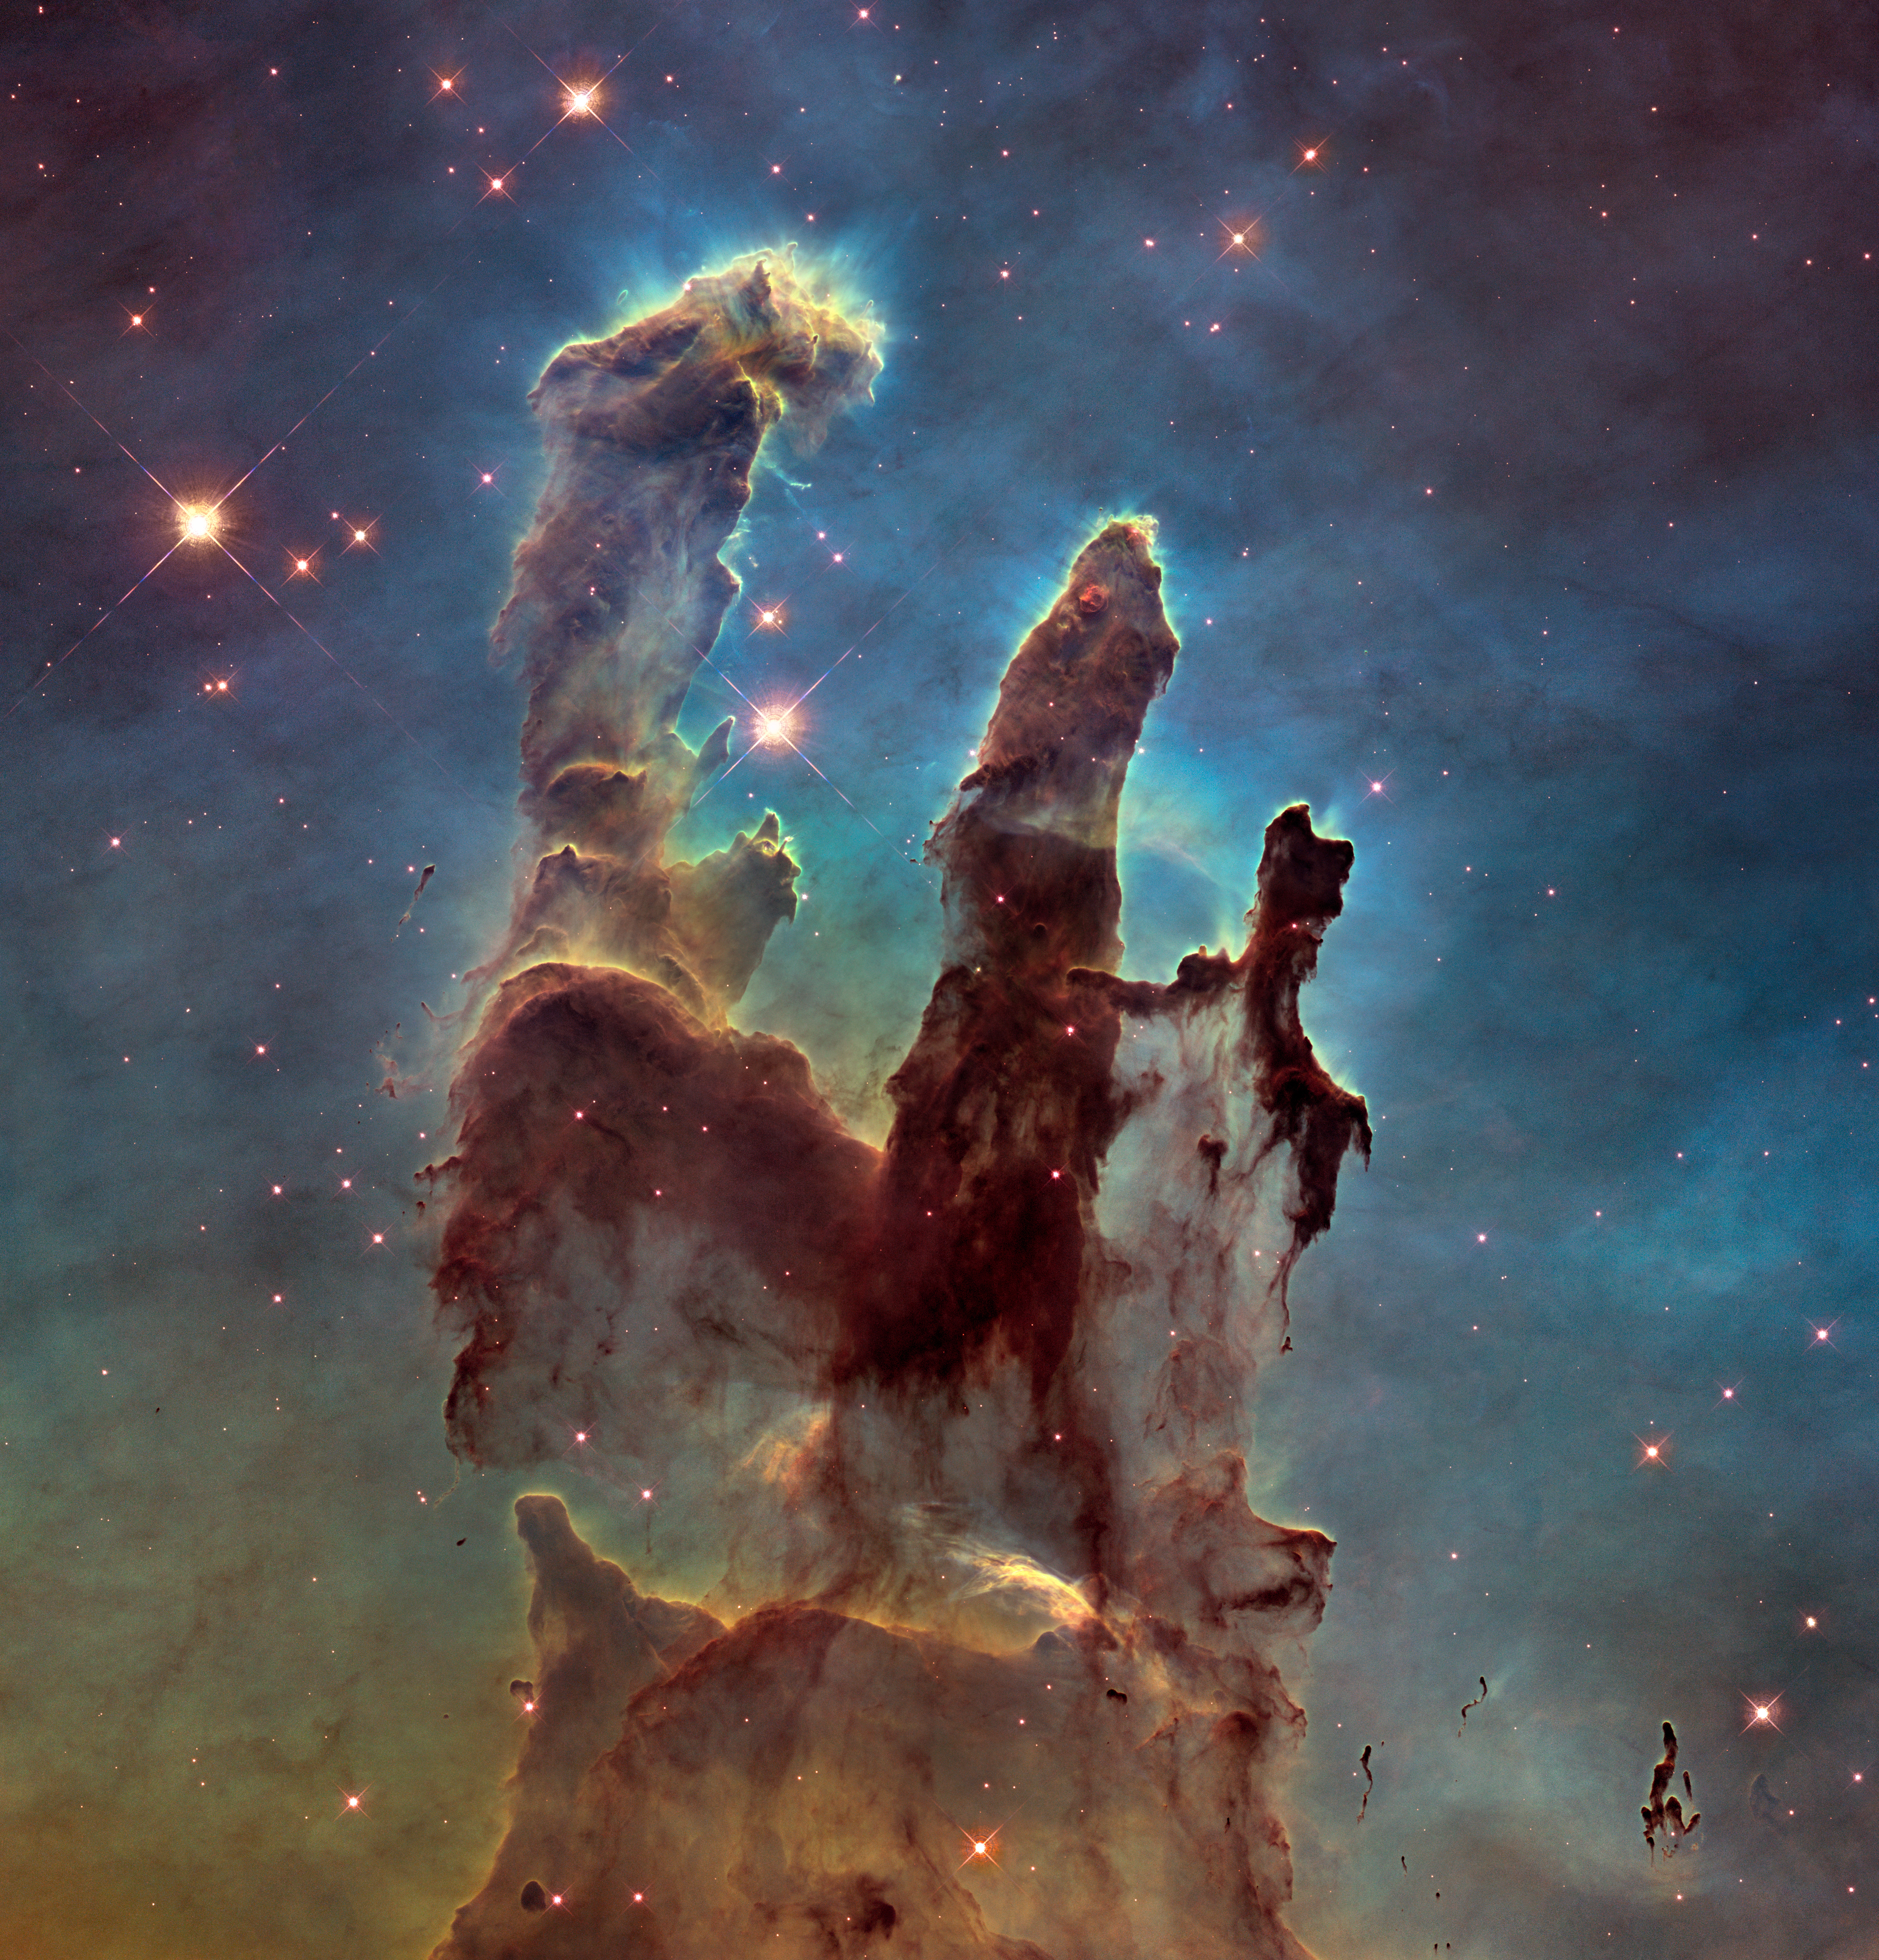
\includegraphics[width=0.6\textwidth]{heic1501a.jpg}}} \\
		\multicolumn{2}{c}{(a)} \\
		\FramePic{\includegraphics[width=0.45\textwidth]{ex-03-pillars-blurred}} &
		\FramePic{\includegraphics[width=0.45\textwidth]{ex-03-pillars-rld-result}} \\
		(b) & (c)
	\end{tabular}
	\caption{Eingabe-Bild~(a); Gefiltertes Bild (Gauss; $\sigma=3.0$)~(b); Rekonstruiertes Bild~(c); Anzahl-Iterationen: 2200; Erwartetes Ergebnis: Rekonstruktion von Bilddetails; Ergebnis: Bilddetails werden fast vollständig wieder hergestellt.}
	\label{ex-03-pillars}
\end{figure}

\begin{figure}[h]
	\centering\small
	\begin{tabular}{cc}
		\multicolumn{2}{c}{\FramePic{\includegraphics[width=0.7\textwidth]{opo1000a.jpg}}} \\
		\multicolumn{2}{c}{(a)} \\
		\FramePic{\includegraphics[width=0.45\textwidth]{ex-04-galaxy-blurred}} &
		\FramePic{\includegraphics[width=0.45\textwidth]{ex-04-galaxy-rld-result}} \\
		(b) & (c)
	\end{tabular}
	\caption{Eingabe-Bild~(a); Gefiltertes Bild (Gauss; $\sigma=16.0$)~(b); Rekonstruiertes Bild~(c); Anzahl-Iterationen: 8000; Erwartetes Ergebnis: Rekonstruktion von Bilddetails; Ergebnis: Bilddetails werden deutlich verbessert aber nicht vollständig wieder hergestellt.}
	\label{ex-04-galaxy}
\end{figure}

\begin{figure}[h]
	\centering\small
	\begin{tabular}{cc}
		\multicolumn{2}{c}{\FramePic{\includegraphics[width=0.7\textwidth]{opo1000a.jpg}}} \\
		\multicolumn{2}{c}{(a)} \\
		\FramePic{\includegraphics[width=0.45\textwidth]{ex-05-galaxy-blurred}} &
		\FramePic{\includegraphics[width=0.45\textwidth]{ex-05-galaxy-rld-result}} \\
		(b) & (c)
	\end{tabular}
	\caption{Eingabe-Bild~(a); Gefiltertes Bild (Gauss; $\sigma=1.8$)~(b); Rekonstruiertes Bild~(c); Anzahl-Iterationen: 800; Erwartetes Ergebnis: Rekonstruktion von Bilddetails; Ergebnis: Bilddetails werden fast vollständig wieder hergestellt.}
	\label{ex-05-galaxy}
\end{figure}


\begin{figure}[h]
	\centering\small
	\begin{tabular}{cc}
		\multicolumn{2}{c}{\FramePic{\includegraphics[width=0.7\textwidth]{STScI-01EVVD1G3V0B3TY7J779XY5W1F.jpg}}} \\
		\multicolumn{2}{c}{(a)} \\
		\FramePic{\includegraphics[width=0.45\textwidth]{ex-07-deep-field-blurred}} &
		\FramePic{\includegraphics[width=0.45\textwidth]{ex-07-deep-field-rld-reconstructed}} \\
		(b) & (c)
	\end{tabular}
	\caption{Eingabe-Bild~(a); Gefiltertes Bild (Gauss; $\sigma=12.0$)~(b); Rekonstruiertes Bild~(c); Anzahl-Iterationen: 12000; Erwartetes Ergebnis: Rekonstruktion von Bilddetails; Ergebnis: Bilddetails werden deutlich verbessert aber nicht vollständig wieder hergestellt (leichte Artefakte erkennbar).}
	\label{ex-07-deep-field}
\end{figure}

% ---------------------------------------------------------------
% ---------------------------------------------------------------

\clearpage

\subsubsection{RLD als Schärfefilter}

Bei diesem Test wird evaluiert inwiefern sich die Richardson-Lucy-Deconvolution zum schärfen von Bildern eignet. Dazu wurde RLD mit einem kleinen Gauss-Kernel angewandt; ohne Vorverarbeitung (Weichzeichnung) wie in den vorgehenden Tests.

\begin{figure}[h]
	\centering\small
	\begin{tabular}{c}
		\FramePic{\includegraphics[width=0.7\textwidth]{ex-04-galaxy-input}} \\
		(a) \\
		\FramePic{\includegraphics[width=0.7\textwidth]{ex-06-galaxy-rld-result-sharpened}} \\
		(b)
	\end{tabular}
	\caption{Eingabe-Bild~(a); Gefiltertes Bild (Gauss; $\sigma=0.5$)~(b); Erwartetes Ergebnis: Verbesserter Mikrokontrast und ein besserer Schärfeeindruck; Ergebnis: Leichte Verbesserung des subjektiven Schärfeeindrucks; Bild wirkt nach dem Filtern noch "natürlich" (keine Artefakte).}
	\label{ex-06-galaxy}
\end{figure}

\begin{figure}[h]
	\centering\small
	\begin{tabular}{c}
		\FramePic{\includegraphics[width=0.7\textwidth]{STScI-01EVVD1G3V0B3TY7J779XY5W1F.jpg}} \\
		(a) \\
		\FramePic{\includegraphics[width=0.7\textwidth]{ex-08-deep-field-rld-sharpened}} \\
		(b)
	\end{tabular}
	\caption{Eingabe-Bild~(a); Gefiltertes Bild (Gauss; $\sigma=0.6$)~(b); Erwartetes Ergebnis: Verbesserter Mikrokontrast und ein besserer Schärfeeindruck; Ergebnis: Leichte Verbesserung des subjektiven Schärfeeindrucks; Bild wirkt nach dem Filtern noch "natürlich" (leichte Artefakte / Rauschen).}
	\label{ex-08-deep-field}
\end{figure}

\begin{figure}[h]
	\centering\small
	\begin{tabular}{c}
		\FramePic{\includegraphics[width=0.7\textwidth]{STScI-01EVVD1G3V0B3TY7J779XY5W1F.jpg}} \\
		(a) \\
		\FramePic{\includegraphics[width=0.7\textwidth]{ex-08-deep-field-rld-sharpened-2}} \\
		(b)
	\end{tabular}
	\caption{Eingabe-Bild~(a); Gefiltertes Bild (Gauss; $\sigma=1.2$)~(b); Erwartetes Ergebnis: Verbesserter Mikrokontrast und ein besserer Schärfeeindruck; Ergebnis: Verbesserung des subjektiven Schärfeeindrucks; Bild weist nach dem Filtern ein deutlich erhöhtes Rauschen auf; das Bild macht subjektiv noch einen "nätürlichen" Eindruck und wirkt als wäre es mit einem hohen ISO-Wert der Kamera aufgenommen worden.}
	\label{ex-09-deep-field}
\end{figure}

% ---------------------------------------------------------------
% ---------------------------------------------------------------

\clearpage

\subsubsection{Unterschiedliche Kernel}

Bei diesem Test wird der Einfluss des verwendeten Kernel auf die zu erwartenden Ergebnisse evaluiert.


\begin{figure}[h]
	\centering\small
	\begin{tabular}{cc}
		\multicolumn{2}{c}{\FramePic{\includegraphics[width=0.6\textwidth]{ex-10-lena-orig}}} \\
		\multicolumn{2}{c}{(a)} \\
		\FramePic{\includegraphics[width=0.45\textwidth]{ex-10-lena-blur}} &
		\FramePic{\includegraphics[width=0.45\textwidth]{ex-10-lena-rld}} \\
		(b) & (c)
	\end{tabular}
	\caption{Eingabe-Bild~(a); Gefiltertes Bild (7x7 Mean)~(b); Rekonstruiertes Bild~(c); Anzahl-Iterationen: 500; Erwartetes Ergebnis: Rekonstruktion von Bilddetails; Ergebnis: Bilddetails werden fast vollständig wieder hergestellt, es sind allerdings Artefakte erkennbar (tendentiell stärker als beim Gauss-Filter).}
	\label{ex-10-lena}
\end{figure}

\begin{figure}[h]
	\centering\small
	\begin{tabular}{cc}
		\multicolumn{2}{c}{\FramePic{\includegraphics[width=0.4\textwidth]{ex-10-lena-orig}}} \\
		\multicolumn{2}{c}{(a)} \\
		\FramePic{\includegraphics[width=0.45\textwidth]{ex-11-lena-blur}} &
		\FramePic{\includegraphics[width=0.45\textwidth]{ex-11-lena-rld}} \\
		(b) & (c)
	\end{tabular}
	\caption{Eingabe-Bild~(a); Gefiltertes Bild (leicht weichgezeichneter Kreis)~(b); Rekonstruiertes Bild~(c); Anzahl-Iterationen: 500; Erwartetes Ergebnis: Rekonstruktion von Bilddetails; Ergebnis: Bilddetails werden fast vollständig wieder hergestellt, es sind allerdings Artefakte erkennbar (tendentiell stärker als beim Gauss-Filter).}
	\label{ex-11-lena}
\end{figure}

\begin{figure}[h]
	\centering\small
	\begin{tabular}{cc}
		\multicolumn{2}{c}{\FramePic{\includegraphics[width=0.4\textwidth]{ex-10-lena-orig}}} \\
		\multicolumn{2}{c}{(a)} \\
		\FramePic{\includegraphics[width=0.45\textwidth]{ex-16-lena-blur}} &
		\FramePic{\includegraphics[width=0.45\textwidth]{ex-16-lena-rld}} \\
		(b) & (c)
	\end{tabular}
	\caption{Eingabe-Bild~(a); Gefiltertes Bild (21x1 Mean)~(b); Rekonstruiertes Bild~(c); Anzahl-Iterationen: 100; Erwartetes Ergebnis: Rekonstruktion von Bilddetails; Ergebnis: Einige Bilddetails können wieder hergestellt, es sind allerdings Artefakte erkennbar (Doppelbilder).}
	\label{ex-15-lena}
\end{figure}

% ---------------------------------------------------------------
\subsubsection{Nicht übereinstimmende Kernel}

Bei diesem Test wird evaluiert, wie gut das Eingangs-Bild Rekonstruiert werden kann, wenn der Kernel zum "weichzeichnen" und für die RLD nicht übereinstimmen.

\begin{figure}[h]
	\centering\small
	\begin{tabular}{cc}
		\FramePic{\includegraphics[width=0.45\textwidth]{ex-17-bridge-blur}} &
		\FramePic{\includegraphics[width=0.45\textwidth]{ex-17-bridge-rld}} \\
		(a) & (b)
	\end{tabular}
	\caption{Gefiltertes Bild (Gauss $\sigma=2.0$)~(a); Rekonstruiertes Bild (Gauss $\sigma=3.0$)~(b); Anzahl-Iterationen: 100; Erwartetes Ergebnis: "Überschärftes" Bild; Ergebnis: leichte Verbesserung der Details, aber starke Artefaktbildung bzw. Überzeichnung / Überschärfung.}
	\label{ex-17-bridge}
\end{figure}

\begin{figure}[h]
	\centering\small
	\begin{tabular}{cc}
		\FramePic{\includegraphics[width=0.45\textwidth]{ex-18-bridge-blur}} &
		\FramePic{\includegraphics[width=0.45\textwidth]{ex-18-bridge-rld}} \\
		(a) & (b)
	\end{tabular}
	\caption{Gefiltertes Bild (Gauss $\sigma=3.0$)~(a); Rekonstruiertes Bild (Gauss $\sigma=2.0$)~(b); Anzahl-Iterationen: 400; Erwartetes Ergebnis: Rekonstruktion von Bilddetails, verbleibende Unschärfe; Ergebnis: leichte Verbesserung der Details, keine Artefaktbildung, das Bild bleibt aber relativ unscharf verglichen mit den Ergebnissen bei denen die Kernel perfekt übereinstimmen.}
	\label{ex-18-bridge}
\end{figure}


\clearpage

% ---------------------------------------------------------------

\subsubsection{Einfluss von Rauschen}

Bei diesem Test wird der Einfluss von Bildrauschen auf die zu erwartenden Ergebnisse evaluiert. Dazu wird nach der initialen Weichzeichnung normalverteiltes Rauschen hinzugefügt.


\begin{figure}[h]
	\centering\small
	\begin{tabular}{cc}
		\FramePic{\includegraphics[width=0.45\textwidth]{ex-12-lena-blur}} &
		\FramePic{\includegraphics[width=0.45\textwidth]{ex-12-lena-rld}} \\
		(a) & (b)
	\end{tabular}
	\caption{Gefiltertes Bild (Gauss $\sigma=3.0$ + Noise ($stddev=10$))~(a); Rekonstruiertes Bild~(b); Anzahl-Iterationen: 500; Erwartetes Ergebnis: Rekonstruktion von Bilddetails; Ergebnis: sehr starke Artefaktbildung.}
	\label{ex-12-lena}
\end{figure}

\begin{figure}[h]
	\centering\small
	\begin{tabular}{cc}
		\FramePic{\includegraphics[width=0.45\textwidth]{ex-13-galaxy-blur}} &
		\FramePic{\includegraphics[width=0.45\textwidth]{ex-13-galaxy-rld}} \\
		(a) & (b)
	\end{tabular}
	\caption{Gefiltertes Bild (Gauss $\sigma=6.0$ + Noise ($stddev=5$))~(a); Rekonstruiertes Bild~(b); Anzahl-Iterationen: 250; Erwartetes Ergebnis: Rekonstruktion von Bilddetails; Ergebnis: leichte Verbesserung der Details, aber auch starke Artefaktbildung.}
	\label{ex-13-galaxy}
\end{figure}

\begin{figure}[h]
	\centering\small
	\begin{tabular}{cc}
		\multicolumn{2}{c}{\FramePic{\includegraphics[width=0.45\textwidth]{ex-19-pillars-blur}}} \\
		\multicolumn{2}{c}{(a)} \\
		\FramePic{\includegraphics[width=0.45\textwidth]{ex-19-pillars-rld-100}} &
		\FramePic{\includegraphics[width=0.45\textwidth]{ex-19-pillars-rld-400}} \\
		(b) & (c)
	\end{tabular}
	\caption{Gefiltertes Bild (Gauss; $\sigma=6.0$ + Noise ($stddev=2$))~(a); Rekonstruiertes Bild (100 Iterationen)~(b); Rekonstruiertes Bild (400 Iterationen)~(c); Anzahl-Iterationen: 100; Erwartetes Ergebnis: Rekonstruktion von Bilddetails; Ergebnis: Einige Bilddetails können wieder hergestellt, es sind allerdings Artefakte erkennbar; Artefaktbildung wird ab ca. Iteration 100 stärker.}
	\label{ex-19-pillars}
\end{figure}

\clearpage

\subsubsection{Unterschiedliche "Startbilder"}

Bei diesem Test wird der Einfluss des initial gewählten "Schätzwerts" auf die zu erwartenden Ergebnisse evaluiert. Dazu wird der Schätzwert auf unterschiedliche Weise initialisiert. Alle vorgehenden Testbilder wurden mit dem weichgezeichneten Bild initialisiert.

\begin{figure}[h]
	\centering\small
	\begin{tabular}{cc}
		\multicolumn{2}{c}{\FramePic{\includegraphics[width=0.45\textwidth]{ex-14-bridge-0}}} \\
		\multicolumn{2}{c}{(a)} \\
		\FramePic{\includegraphics[width=0.45\textwidth]{ex-14-bridge-1}} &
		\FramePic{\includegraphics[width=0.45\textwidth]{ex-14-bridge-2}} \\
		(b) & (c)
	\end{tabular}
	\caption{Iteration 0~(a); Iteration 1~(b); Iteration 2~(c); Erwartetes Ergebnis: "Schwarzes Bild" das nach mehreren Iterationen immer mehr dem Eingabe-Bild ("Bridge") entspricht; Ergebnis: schon nach der ersten Iteration des Algorithmus ist das Eingabe-Bild deutlich erkennbar.}
	\label{ex-14-bridge}
\end{figure}

\begin{figure}[h]
	\centering\small
	\begin{tabular}{cc}
		\FramePic{\includegraphics[width=0.45\textwidth]{ex-15-bridge-0}} &
		\FramePic{\includegraphics[width=0.45\textwidth]{ex-15-bridge-1}} \\
		(a) & (b) \\
		\FramePic{\includegraphics[width=0.45\textwidth]{ex-15-bridge-10}} &
		\FramePic{\includegraphics[width=0.45\textwidth]{ex-15-bridge-100}} \\
		(c) & (d)
	\end{tabular}
	\caption{Iteration 0~(a); Iteration 1~(b); Iteration 10~(c); Iteration 100~(d); Erwartetes Ergebnis: "Verrauschtes Bild" das nach mehreren Iterationen immer mehr dem Eingabe-Bild ("Bridge") entspricht; Ergebnis: Es dauert enorm lange bis das gleichverteilte Rauschen annähernd dem Eingabe-Bild entspricht.}
	\label{ex-15-bridge}
\end{figure}

% \begin{figure}[h]
% \centering
% \includegraphics[width=.7\textwidth]{test-01-A}
% \caption{Alle 'A' im Bild markiert.}
% \label{fig:test-01}
% \end{figure}

\clearpage

\subsection{Erkenntnisse}

Die Parameter haben teils einen sehr großen Einfluss auf die Qualität der Ergebnisse. Mit gut gewählten Parametern können "erstaunlich" gute Rekonstruktionen realisiert werden, vorallem für einen -- zumindest in der Implementierung -- simplen Algorithmus.

%%%-----------------------------------------------------------------------------

% \section{Titel der zweiten Aufgabe}

%%%-----------------------------------------------------------------------------

%\section*{Zusammenfassung und Anmerkungen}

%%%-----------------------------------------------------------------------------

% \section*{Quellen}

% \printbibliography[heading=noheader]

%%%-----------------------------------------------------------------------------
\end{document}
%%%-----------------------------------------------------------------------------